\documentclass[tikz, border=1mm]{standalone}

\usetikzlibrary{positioning}

\begin{document}
	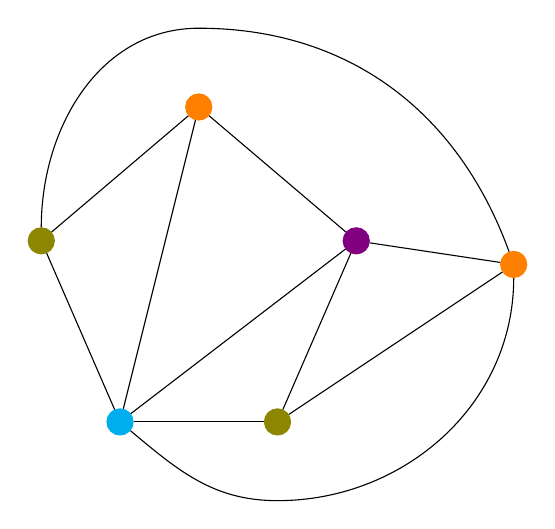
\begin{tikzpicture}[main/.style = {draw, circle, fill}]
		\node[main, color = cyan] (1) at (0,0) {};
		\node[main, color = olive] (2) at (2,0) {};
		\node[main, color = olive] (3) at (-1, 2.3) {};
		\node[main, color = violet] (4) at (3, 2.3) {};
		\node[main, color = orange] (5) at (1, 4) {};
		\node[main, color = orange] (6) at (5, 2) {};
		\draw (1) -- (2);
		\draw (1) -- (3);
		\draw (2) -- (4);
		\draw (3) -- (5);
		\draw (4) -- (5);
		\draw (1) -- (4);
		\draw (1) -- (5);
		\draw (4) -- (6);
		\draw (2) -- (6);
		\draw (1) to[out = -40, in = 180] (2,-1) to[out = 0, in = -90] (6);
		\draw (3) to[out = 90, in = 180] (1, 5) to[out = 0, in = 110] (6);
	\end{tikzpicture}
\end{document}